\documentclass[12pt, a4paper]{article}
\usepackage{amsmath}
\usepackage{amssymb}
\usepackage{tikz}
\usepackage{xcolor}

\begin{document}

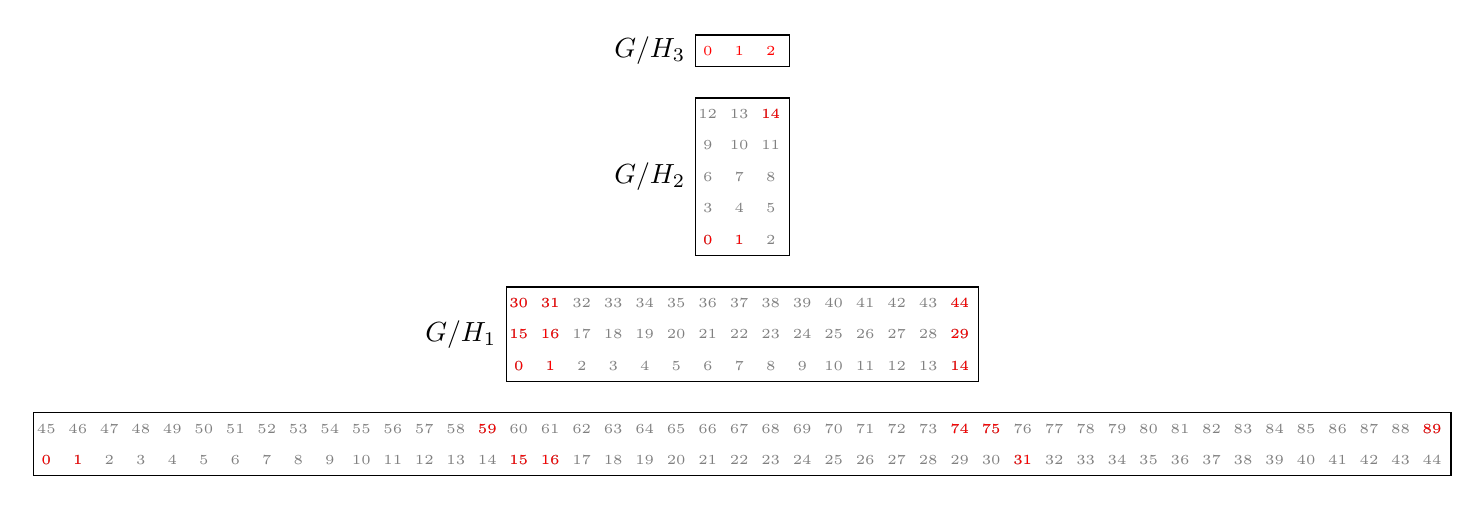
\begin{tikzpicture}[scale=0.4]
\draw (-22.5,0) rectangle (22.5,2);
\foreach \i in {0,...,44}
{
\node[gray] at (\i+0.4-22.5,0.5) {\tiny\i};
}
\foreach \i in {45,...,89}
{
\node[gray] at (\i+0.4-45-22.5,1.5) {\tiny\i};
}
\node[red] at (0.4-22.5,0.5) {\tiny 0};
\node[red] at (0.4-22.5+1,0.5) {\tiny 1};
\node[red] at (0.4-22.5+15,0.5) {\tiny 15};
\node[red] at (0.4-22.5+16,0.5) {\tiny 16};
\node[red] at (0.4-22.5+31,0.5) {\tiny 31};
\node[red] at (0.4-22.5+14,1.5) {\tiny 59};
\node[red] at (0.4-22.5+29,1.5) {\tiny 74};
\node[red] at (0.4-22.5+30,1.5) {\tiny 75};
\node[red] at (0.4-22.5+44,1.5) {\tiny 89};

%0,1,89,15,75,16,74,31,59
%%%%%%%%%%%%%%%%%%%%%
\draw (-7.5,3) rectangle (7.5,6);
\foreach \i in {0,...,14}
{
\node[gray] at (\i+0.4-7.5,3.5) {\tiny \i};
}
\foreach \i in {15,...,29}
{
\node[gray] at (\i+0.4-7.5-15,4.5) {\tiny \i};
}
\foreach \i in {30,...,44}
{
\node[gray] at (\i+0.4-7.5-30,5.5) {\tiny \i};
}
\node[red] at (0.4-7.5,3.5) {\tiny 0};
\node[red] at (0.4-7.5,4.5) {\tiny 15};
\node[red] at (0.4-7.5,5.5) {\tiny 30};

\node[red] at (0.4-6.5,3.5) {\tiny 1};
\node[red] at (0.4-6.5,4.5) {\tiny 16};
\node[red] at (0.4-6.5,5.5) {\tiny 31};

\node[red] at (0.4+6.5,3.5) {\tiny 14};
\node[red] at (0.4+6.5,4.5) {\tiny 29};
\node[red] at (0.4+6.5,5.5) {\tiny 44};

\node[left] at (-7.5,4.5) {$G/H_1$};
%%%%%%%%%%%%%%%%%%%%%
\draw (-1.5, 7) rectangle (1.5,12);
\foreach \i in {0,1,2}
\node[gray] at (\i+0.4-1.5, 7.5) {\tiny \i};
\foreach \i in {3,4,5}
\node[gray] at (\i+0.4-1.5-3, 8.5) {\tiny \i};
\foreach \i in {6,7,8}
\node[gray] at (\i+0.4-1.5-6, 9.5) {\tiny \i};
\foreach \i in {9,10,11}
\node[gray] at (\i+0.4-1.5-9, 10.5) {\tiny \i};
\foreach \i in {12,13,14}
\node[gray] at (\i+0.4-1.5-12, 11.5) {\tiny \i};

\node[red] at (0.4-1.5,7.5) {\tiny 0};
\node[red] at (0.4-1.5+1,7.5) {\tiny 1};
\node[red] at (0.4-1.5+2,11.5) {\tiny 14};

\node[left] at (-1.5,9.5) {$G/H_2$};
%%%%%%%%%%%%%%%%%%%%
\draw (-1.5,13) rectangle (1.5,14);
\foreach \i in {0,1,2}
\node[red] at (\i+0.4-1.5,13.5) {\tiny \i};
\node[left] at (-1.5,13.5) {$G/H_3$};
\end{tikzpicture}

\end{document}